\section{Web User Interface}
As mentioned in the design section, one of the non-functional requirements is the ease of use of the application. This is to allow anyone without any programming skills to still use ALIAS. Hence, in order to meet this requirement, a web User Interface has been implemented, which is part of the solution.

The back-end of web interface has been implemented using Python Flask micro framework \citep{flaskDocs}. Given the Flask is implemented purely in Python makes one of the most appropriate technologies for the given purpose. Furthermore, the User Interface will be used to upload and create Argumentation Frameworks, add arguments and attacks. Flask also provides the web server and although it meant to be only used for development and testing \citep{flaskBook}, it is perfect for the purpose of running ALIAS locally. ALIAS Web Interface expose certain methods of ALIAS application making it easy to create argumentation frameworks and display required extensions. The Web API exposes following methods from the ALIAS application:
\begin{enumerate}
	\item Load example Argumentation Framework
	\item Upload custom Argumentation Framework in tgf format
	\item Create new Argumentation Framework
	\item Add argument
	\item Add attack
\end{enumerate}

In order to display the Argumentation Framework as a graph in the User Interface, the CytoscapeJS \citep{cytoscapejs} framework has been used with the Cola.js constraint-based layout type. As can be seen in figure \ref{fig:webUi}, those technologies allow for creation of complex directed graphs which are dynamically balanced.

\begin{figure}[h]
	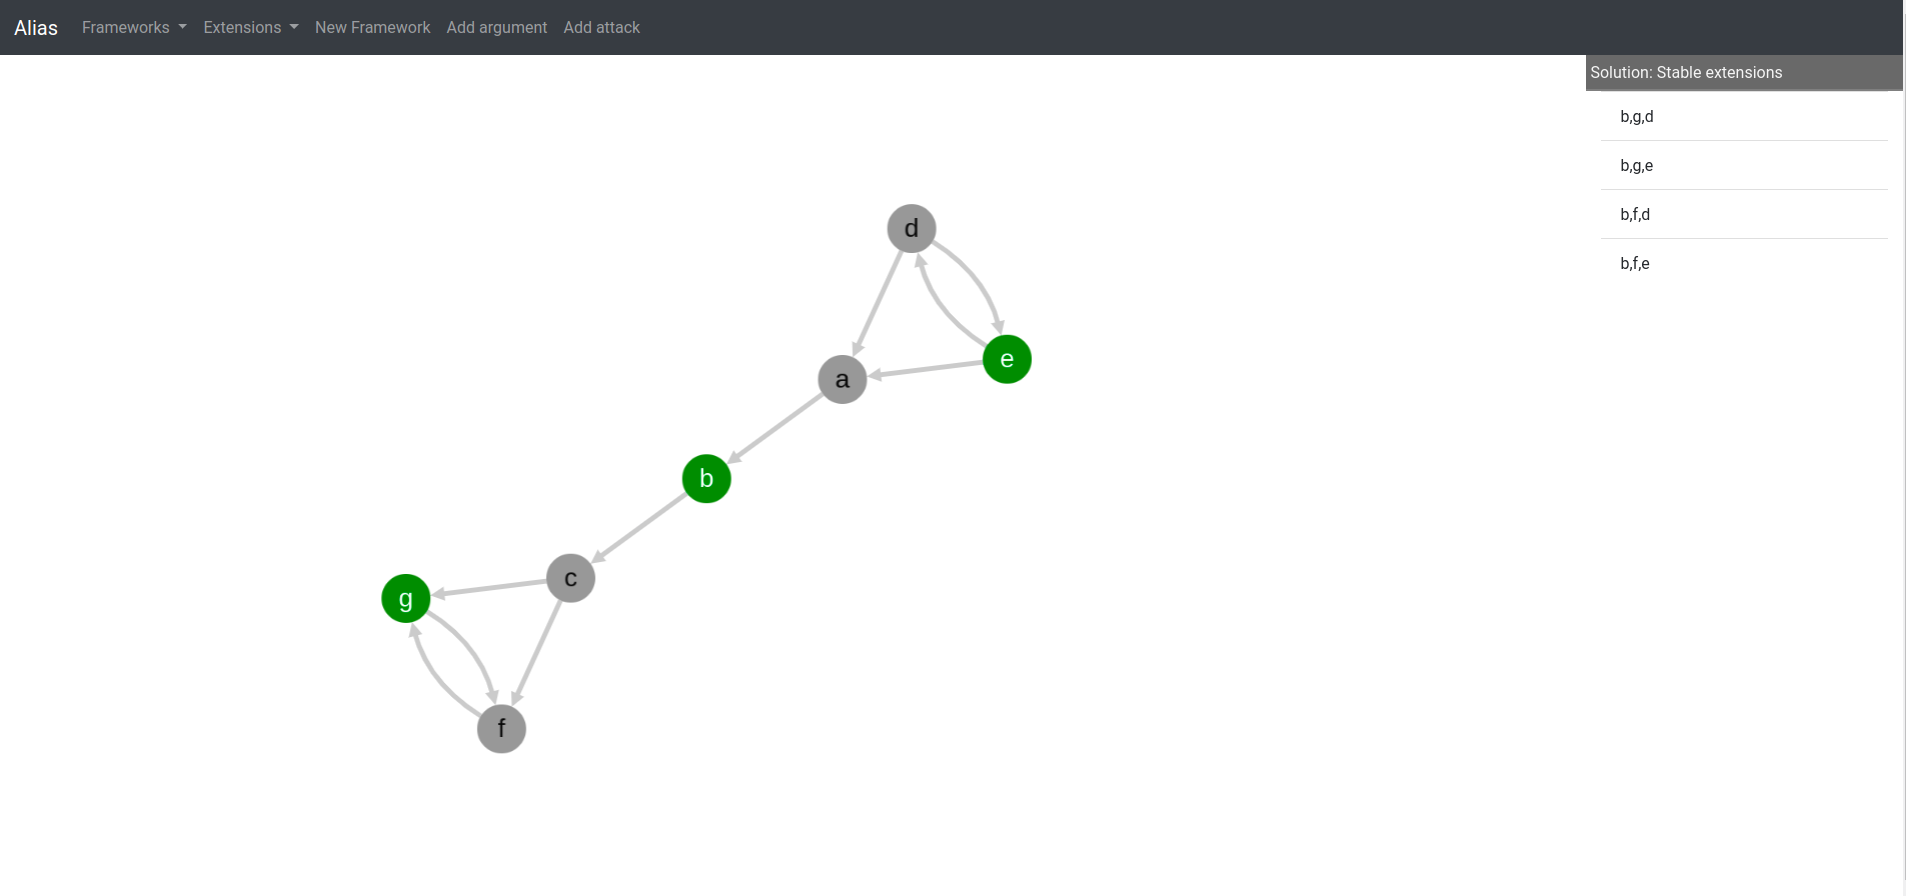
\includegraphics[width=\textwidth]{webui}
	\caption{ALIAS Web User Interface}
	\label{fig:webUi}
\end{figure}

The Web Interface allows the user to upload their own Argumentation Framework in trivial graph format. Although ALIAS can parse Argumentation Frameworks from different file formats like apx or JSON, at the moment the web interface can work only in tgf file format. 

All the user interaction uploading the framework, adding arguments and attacks are done through modal boxes in HTML structure. This can be seen in figures \ref{fig:upload}, \ref{fig:addArgument}, \ref{fig:addAttacks}. Each modal consist of the form that allows the user to either select the file to upload, or enter id of the argument or id of attacking and attacked arguments. Once the form is submitted, the AJAX call is made through JQuery to access the exposed methods from ALIAS. As mentioned above, each method implemented with Flask returns the JSON representation of the current Argumentation Framework. Once the AJAX call is done, the returned framework is rendered in Web Interface using Cytoscape.js.

\begin{figure}[!ht]
	\centering
	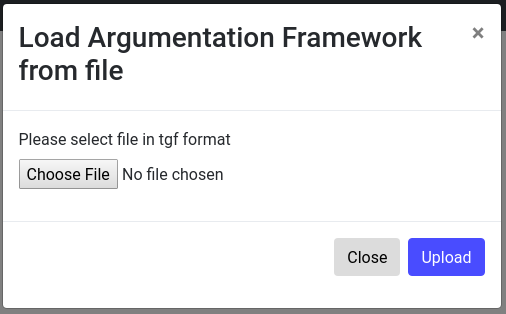
\includegraphics[width=0.7\textwidth]{upload}
	\caption{ALIAS Web User Interface - upload Argumentation Framework modal}
	\label{fig:upload}
\end{figure}

\begin{figure}[h]
	\centering
	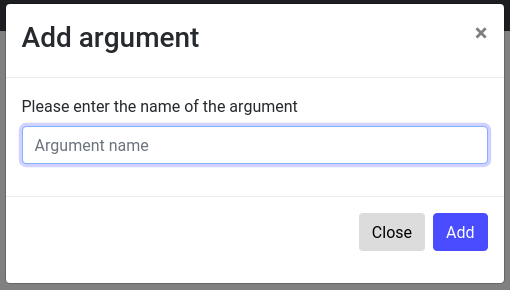
\includegraphics[width=0.7\textwidth]{addArgument}
	\caption{ALIAS Web User Interface - Add Argument modal}
	\label{fig:addArgument}
\end{figure}

\begin{figure}[h]
	\centering
	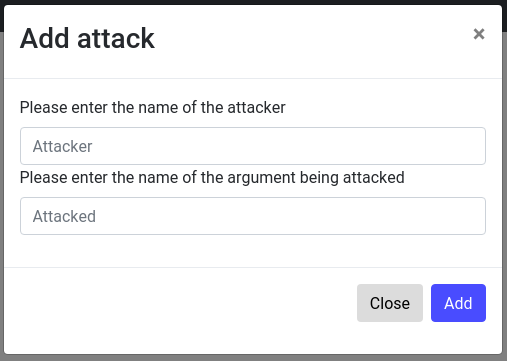
\includegraphics[width=0.7\textwidth]{addAttack}
	\caption{ALIAS Web User Interface - Add Attacks modal}
	\label{fig:addAttacks}
\end{figure}

\subsection{Extensions}
The Web Interface also allows the user to view any possible extensions for the current Argumentation Framework. The available extensions are currently limited by the capabilities of ALIAS. Hence, user can only view all complete, stable and preferred extensions. 

The list of available extensions is provided as a drop-down list in the navigation bar. Once user selects one of extensions, AJAX call is made to ALIAS passing the reference to required semantic. ALIAS computes all the sets for the required semantic and result is returned in the JSON format to the web interface. On receiving the sets from extension, they are rendered as a list on the right hand side of the graph, as shown in figure \ref{fig:webUi}.

User can interact with the given extension results from ALIAS by clicking on any of the item in the solutions list. The selected solution is then displayed on the graph by highlighting the corresponding nodes. This was achieved by changing the class of the nodes with ids corresponding to the ids from the given solution. By highlighting the nodes included in the given solution, the user can clearly see the output from ALIAS.